\documentclass[11pt]{beamer}
\usepackage[utf8]{inputenc}
\usepackage[T1]{fontenc}
\usepackage{amsmath}
\usepackage{amsfonts}
\usepackage{amssymb}
\usepackage{graphicx}
\usepackage[french]{babel}
%\usepackage{siunitx}

%\usepackage{subfig}
\usepackage[squaren,Gray]{SIunits}
\usepackage{array}
\usepackage[french]{babel}
\usepackage{pgfornament}
\usepackage{braket}
\usepackage{blochsphere}
\usepackage{tikz}
\usepackage{mathtools}

\usetikzlibrary{calc}

\usetheme{Pittsburgh}
\usepackage{printlen}
%\usepackage{layouts}

\usefonttheme{serif}

\newcommand{\qb}[2]{\ensuremath{\left|\begin{matrix*}[l]
#1\\[2pt]#2
\end{matrix*}\right>}}


\begin{document}
	\setbeamercovered{transparent}
	\setbeamercolor{institute}{fg=orange!50!red!90}
	\author{Alain Delaet \and André Kalouguine}
	\setbeamercolor{block title}{bg=blue!15,fg=purple}
	\setbeamercolor{block body}{bg=blue!5,fg=black} 
	\setbeamertemplate{sidebar right}{}
	\title{Décohérence des systèmes quantiques uniques}
	\subtitle{\texttt{Systèmes quantiques uniques, trajectoires et décohŕence}}
	\institute{E.N.S. de Lyon}
	\date{22 mai 2018}

	%\setbeamercovered{transparent}
	\setbeamertemplate{footline}{\hspace{0.5em}\insertframenumber\hfill \inserttotalframenumber\hspace{0.5em}}
	\setbeamertemplate{navigation symbols}{}
	\setbeamertemplate{caption}[numbered]
	\addtobeamertemplate{footline}{\vspace{-0.5em}}{\vspace{0.5em}}
	%\addtobeamertemplate{footline}{\vspace{-0.5em}}{\vspace{0.5em}}
	\addtobeamertemplate{headline}{\vspace{.5em}\hspace{.5em}\insertlogo}{}

	\frame{\maketitle}

\begin{frame}{Introduction}
\framesubtitle{Systèmes quantiques uniques}
INCOMPLET IMAGES des differents types de systemes quantiques
\end{frame}

\begin{frame}{Plan}
On utilise QuTiP, une bibliothèque Python pour montrer l'apparition de la décohérence dans des systèmes quantiques simples couplés a l'environnement.
\tableofcontents
\end{frame}

\section{Introduction}


\begin{frame}{Introduction}
\framesubtitle{Oscillateur harmonique}
Pour les systèmes dont l'énergie potentielle a un minimum local, on peut souvent le paraboliser (p.ex molécule diatomique).
On a alors
\[
H_{osc}=\frac{p^2}{2m}+\frac 12 m\omega^2x^2
\]
La résolution de cela montre que l'état du système peut être décrit par un vecteur dans un espace de Hilbert de dimension décomptable:
\[
\left|\begin{matrix}
c_0 \\ c_1 \\ \vdots \\c_n \\ \vdots
\end{matrix}\right.
\]
\end{frame}

\begin{frame}{Introduction}
\framesubtitle{Qubit}
On peut isoler dans certains systèmes deux états privilégiés:\begin{itemize}
\item Spin ($\ket{\uparrow}$ ou $\ket{\downarrow}$)
\item Atome ($\ket{g}$ ou $\ket{e}$)
\item Oscillateur harmonique ($\ket{n}$ ou $\ket{n+1}$)
\item Double puit de potentiel ($\ket{L}$ ou $\ket{R}$)
\item Particule dans une boite ($\ket{\psi_n}$ ou $\ket{\psi_{n+1}}$)
\item $\cdots$
\end{itemize}
L'état du système se décrit alors par un vecteur dans un espace hilbertien de dimension 2: 
\[
\left|\begin{matrix}
\alpha \\ \beta
\end{matrix}\right>
\]
\end{frame}

%\begin{frame}{Introduction}
%\framesubtitle{Qubit et oscillateur couplés}
%Finalement un dernier système simple est un système a deux états couplé a un oscillateur harmonique. C'est un système utile puisque il est utilisé pour controler le qubit par le biais de l'oscillateur. Ce système est décrit par le modèle de Jaynes-Cummings.
%On a alors un système dont l'hamiltonien est:
%\[H_{qb+osc}=H_{osc}\otimes1_{qb}+H_{qb}\otimes1_{osc}+H_{int}
%\]
%\end{frame}

\section{Résolution des systèmes simples}

\begin{frame}{Résolution analytique}
\framesubtitle{Ëquation de Schrödinger}
\end{frame}

\begin{frame}{Qubit}
\framesubtitle{Résolution analytique}
L'hamiltionien devant être hermitien et l'éspace étant de dimension 2, on peut le diagonaliser:
\[
H_{qb}=\begin{bmatrix}
E_0&0\\
0&E_1
\end{bmatrix}
\]
On utilise a partir de cet instant la base propre de l'hamiltonien: $\ket{0}$ et $\ket{1}$.
Ce sont des états stationnaires de pulsations $\omega_0=\frac{E_0}{\hbar}$ et $\omega_1=\frac{E_1}{\hbar}$.\vspace{0.5em}

Si $\ket{\psi(t=0)}=\qb{c_0}{c_1}$ alors $\ket{\psi(t)}=\qb{c_0\cdot\textrm{e}^{i\omega_0 t}}{c_1\cdot\textrm{e}^{i\omega_1 t}}$
\end{frame}

\begin{frame}{Qubit}
\framesubtitle{Visualisation}
L'état d'un qubit est donné par un vecteur de $\mathcal{H}_2(\mathbb{C})$. Modulo la phase totale et en normalisant le vecteur, on peut l'écrire:
\[
\ket{\psi}=\qb{\cos{\frac{\theta}{2}}}{\sin{\frac{\theta}{2}}\cdot\textrm{e}^{i\phi}}
\]
Cela représente un vecteur sur la sphère $\mathcal{S}_3$: la sphère de Bloch.
\begin{figure}
\centering
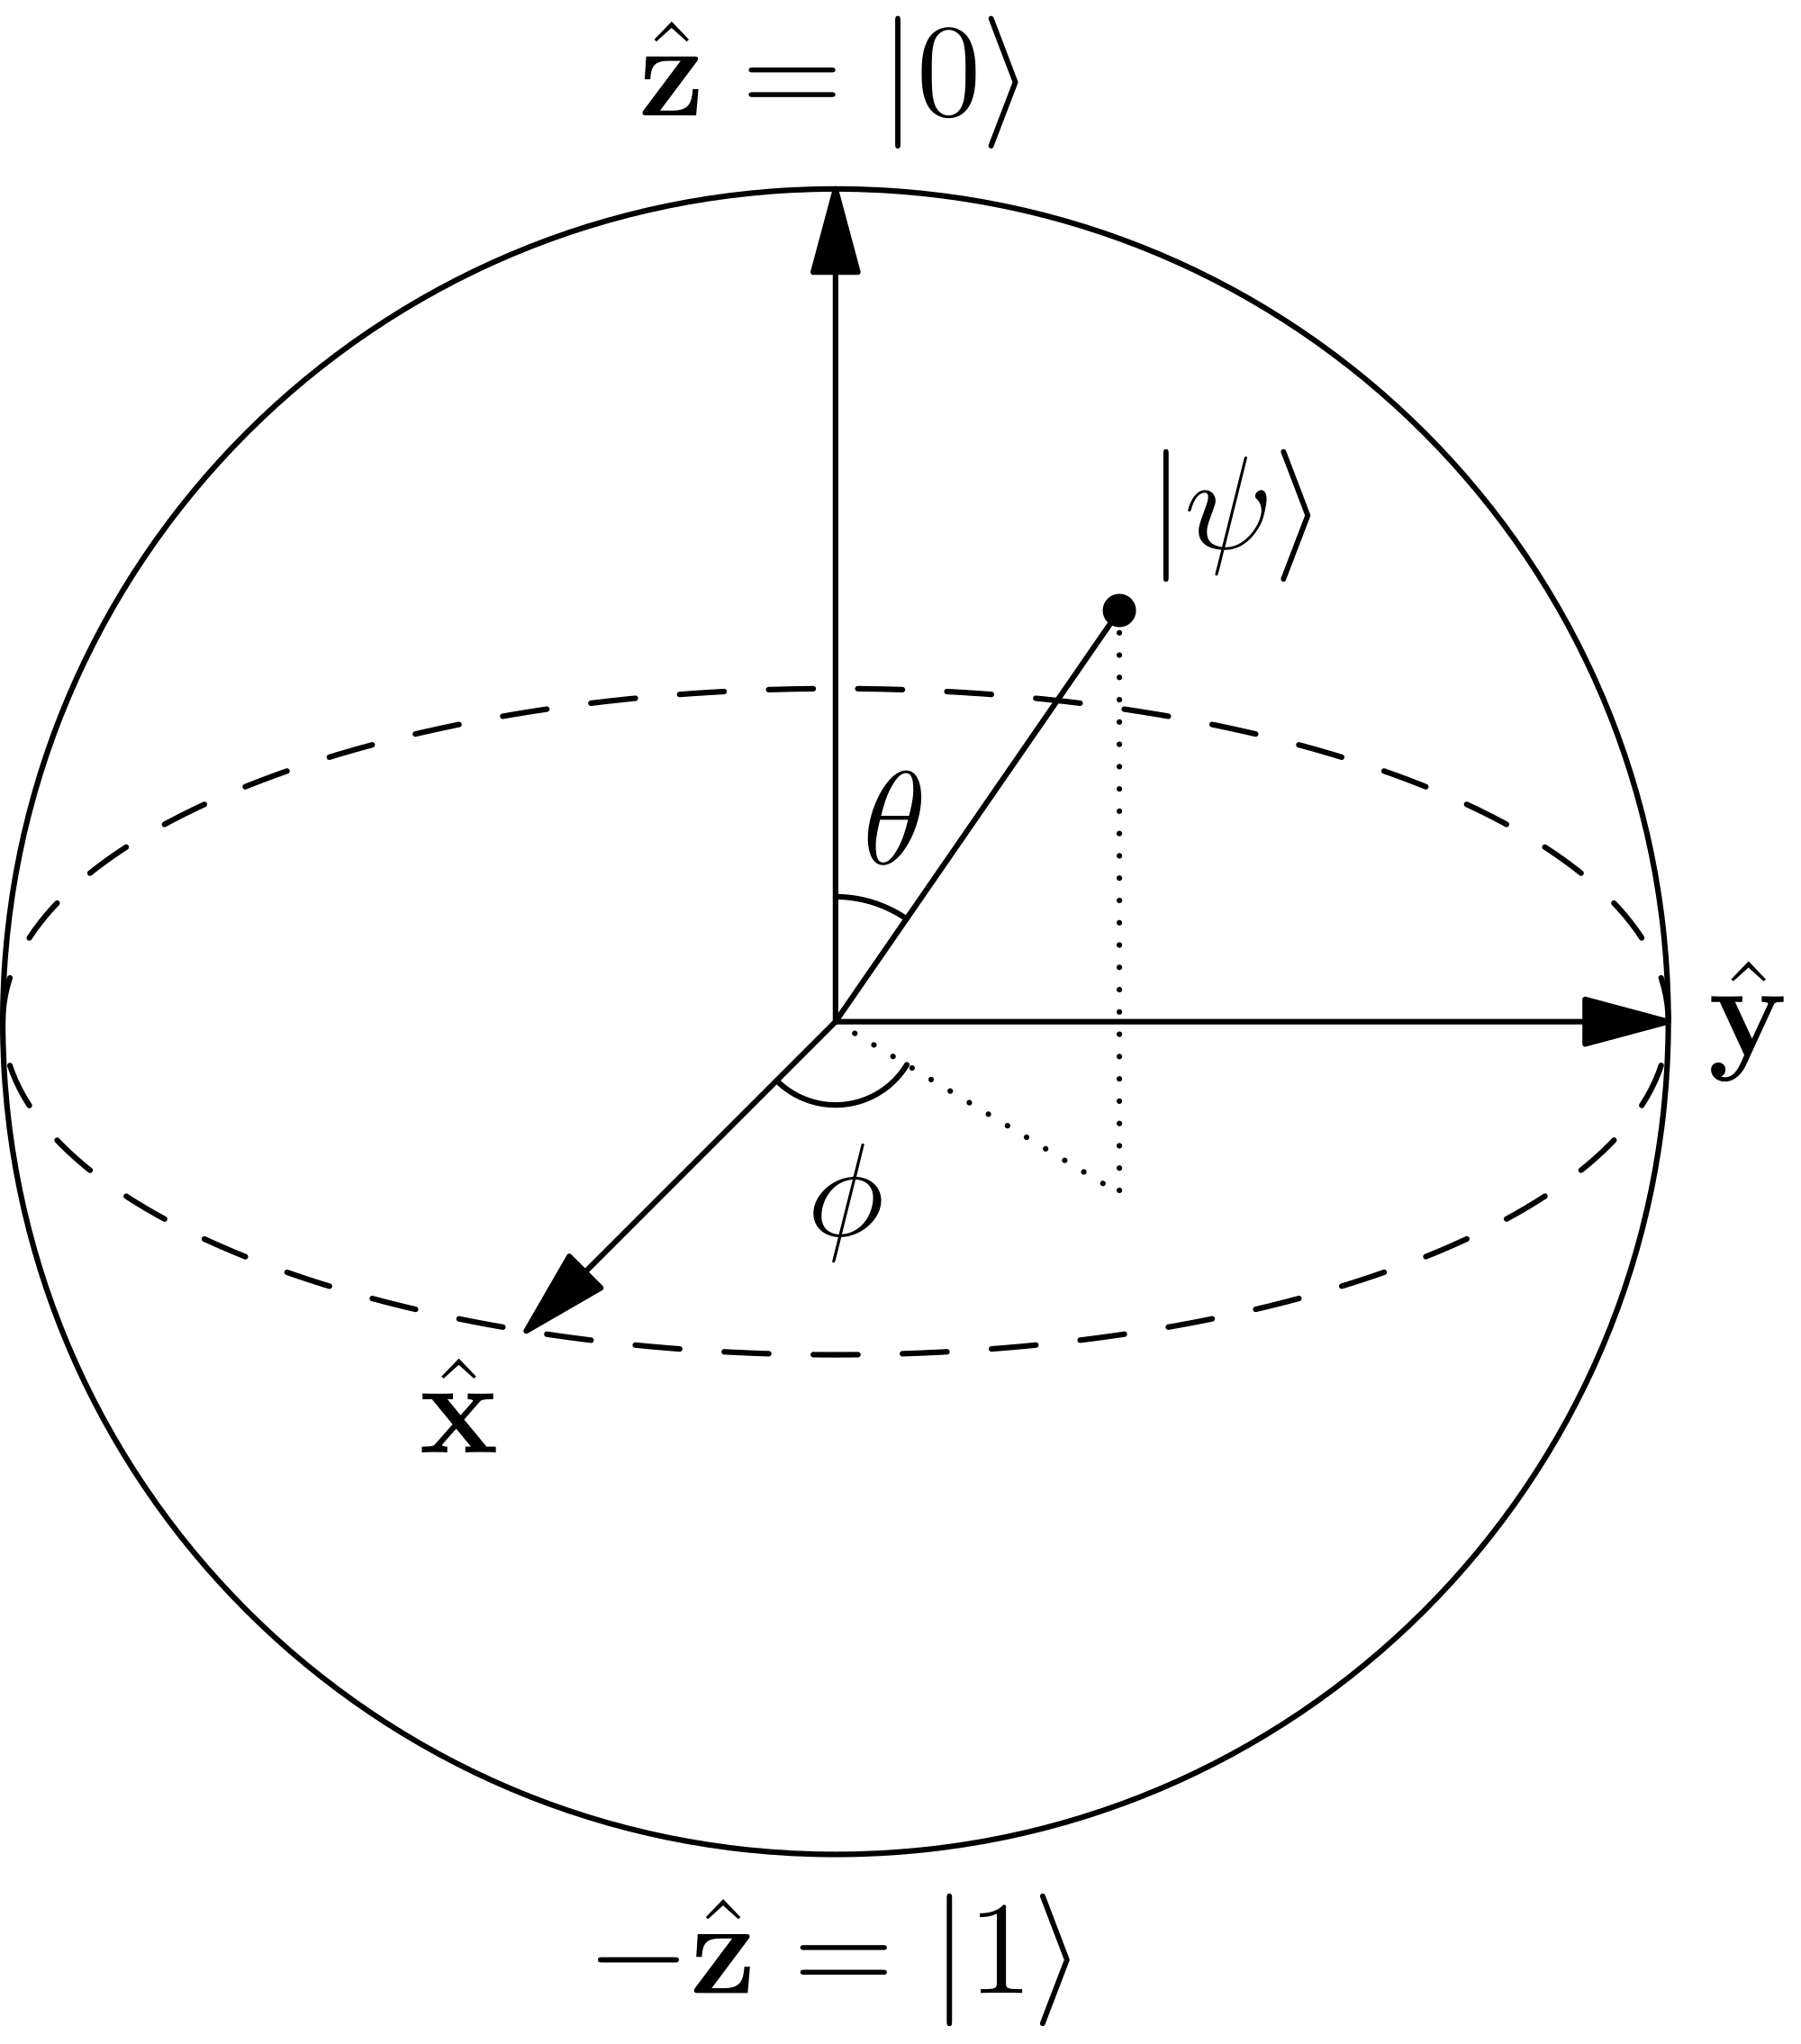
\includegraphics[width=0.3\linewidth]{Bloch_diag}
\end{figure}
\end{frame}

\begin{frame}{Qubit}
\framesubtitle{Oscillations de Rabi}
Si $E_0\neq E_1$, on aura $\omega_0\neq \omega_1$. Modulo la phase totale, on aura donc pour  $\ket{\psi(0)}=\qb{\cos{\frac{\theta}{2}}}{\sin{\frac{\theta}{2}}\cdot\textrm{e}^{i\phi}}$:
\[
\ket{\psi(t)}=\qb{\cos{\frac{\theta}{2}}}{\sin{\frac{\theta}{2}}\cdot\textrm{e}^{i(\phi+\Delta\omega\cdot t)}}
\]
ou $\Delta\omega=\omega_1-\omega_0$.
On a donc le vecteur sur la sphère de Bloch qui tourne autour de l'axe $z$ a une vitesse angulaire $\Delta\omega$.
\end{frame}

\begin{frame}{Qubit}
\framesubtitle{Simulation}
QuTiP a une fonction qui résout l'équation de Schrödinger numériquement: \texttt{mesolve}.
Ainsi, on peut observer les 3 projections sur la sphère de Bloch: $\sigma_x$,$\sigma_y$,$\sigma_z$. On s'attend a voir $x$ et $y$ osciller. 
On a pris ici $\theta=\frac 12$ et $\phi=1$, $\hbar=1$ et $\Delta\omega=1$:

\begin{figure}
\centering
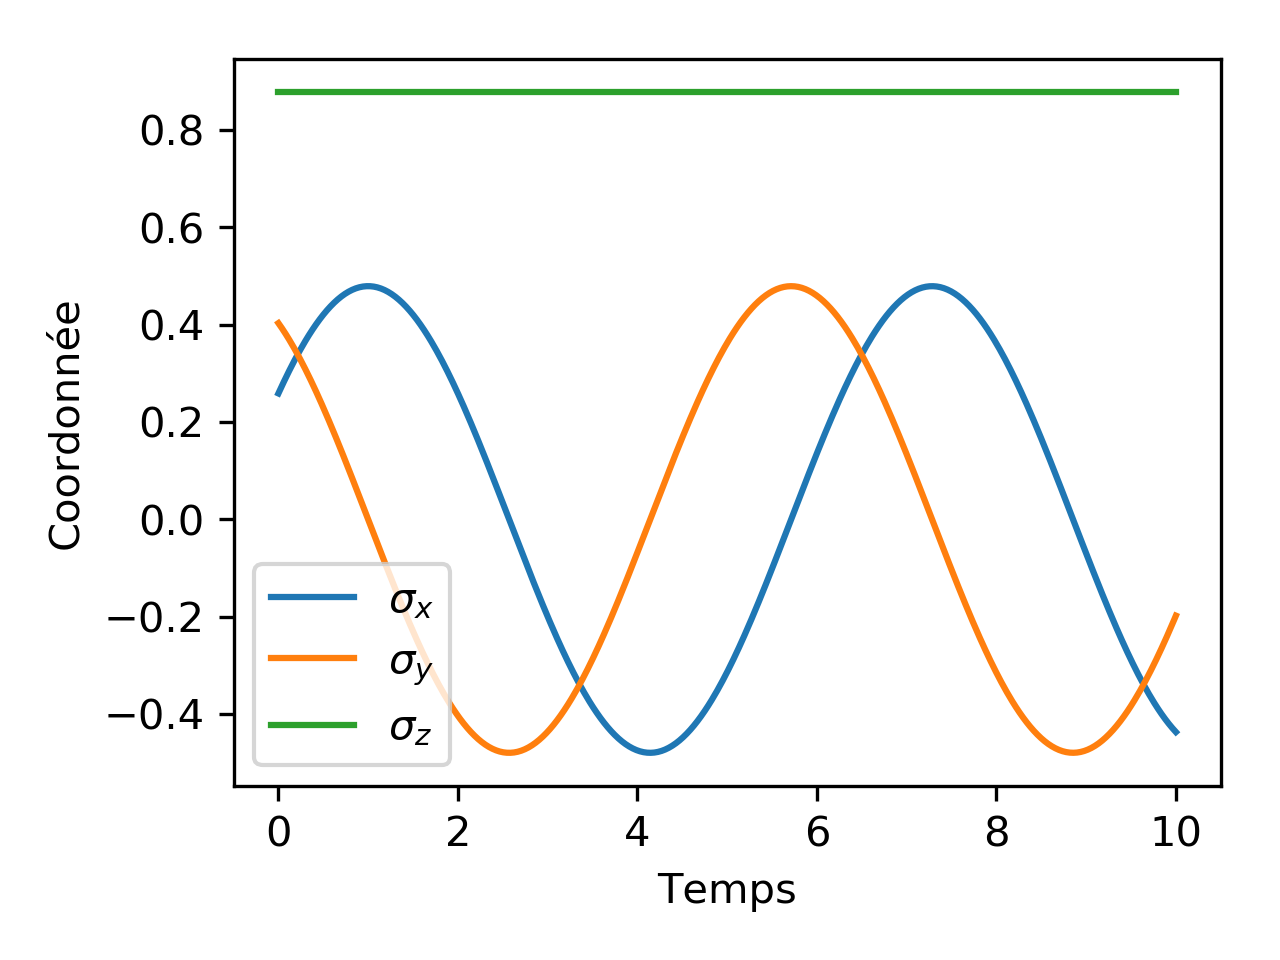
\includegraphics[width=0.7\linewidth]{pres_rabi}
\caption{Oscillations de Rabi}
\label{fig:presrabi}
\end{figure}
\end{frame}

\begin{frame}{Oscillateur harmonique}
\framesubtitle{Résolution analytique}
L'hamiltonien $H_{osc}=\frac{p^2}{2m}+\frac 12 m\omega^2x^2$ peut se réécrire a l'aide de l'opérateur $\displaystyle a=\sqrt{\frac{m\omega}{2\hbar}}\left(x+\frac{i}{m\omega}p\right)$ comme 
\[
H_{osc}=\hbar\omega\left(a^{\dag}a+\frac 12\right)
\]

On pose $\hat{N}=a^{\dag}a$.

$\hat{N}$ se diagonalise et a pour spectre $\mathbb{N}$.

L'état propre de $H_{osc}$ de valeur propre $\hbar\omega(n+\frac 12)$ est $\ket{n}$.
\end{frame}

\begin{frame}{Oscillateur harmonique}
\framesubtitle{Visualisation}
\begin{block}{Fonction de Wigner (sur l'éspace des phases)}
\[
\mathcal{W}(x,p)=\frac{1}{\pi\hbar}\int_{-\infty}^{+\infty}\psi^*(x+y)\psi(x-y)\textrm{e}^{2ipy/\hbar}\textrm{dy}
\]
\end{block}

On a la probabilité de présence en représentation $x$: P(x)=$\int\mathcal{W}(x,p)\textrm{dp}$ et vice versa.

Si négative: état sans analogue classique.
\end{frame}

\begin{frame}{Oscillateur harmonique}
\framesubtitle{Dynamique}
\begin{columns}
\column{0.5\textwidth}
États de Fock:\begin{itemize}
\item Stationnaires
\item Purement quantiques
\end{itemize}

\begin{figure}
\centering
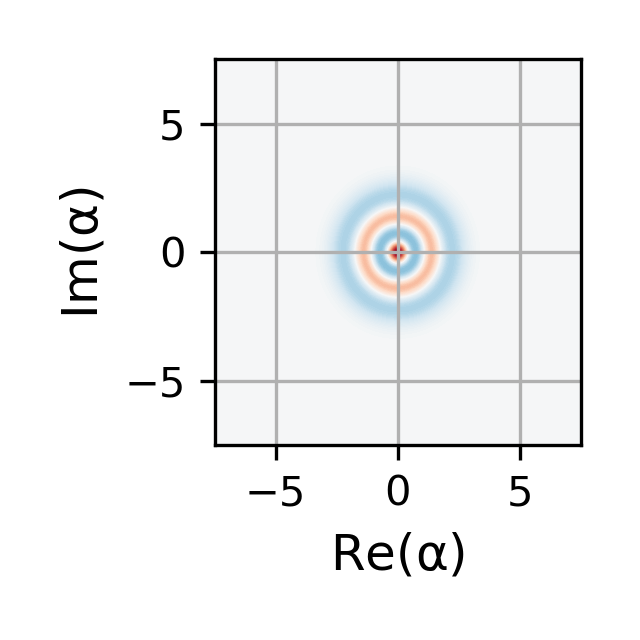
\includegraphics[width=0.7\linewidth]{pres_wigner_fock}
\caption{Etat n=3}
\label{fig:preswignerfock}
\end{figure}

\column{0.5\textwidth}
États cohérents:\begin{itemize}
\item États propres de $a$.
\item Semi classiques: tournent
\end{itemize}

\begin{figure}
\centering
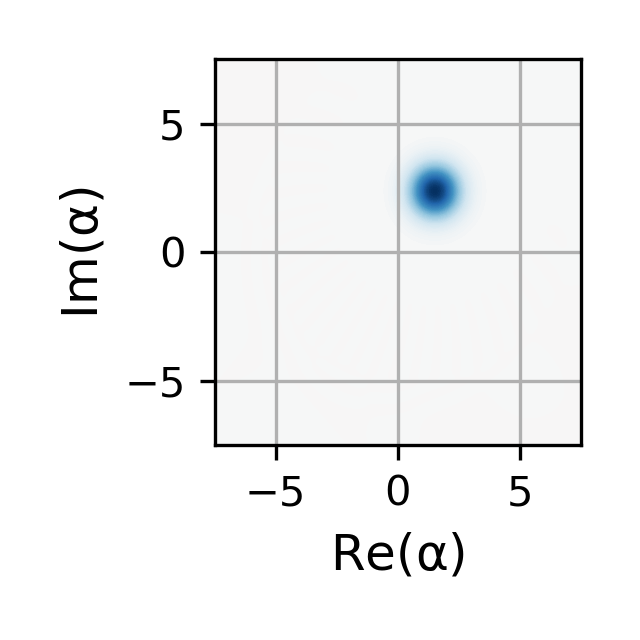
\includegraphics[width=0.7\linewidth]{pres_wigner_coh}
\caption{$\alpha=2\cdot\textrm{e}^{i\cdot1}$}
\label{fig:preswignercoh}
\end{figure}
\end{columns}
\end{frame}

\begin{frame}{Oscillateur harmonique}
\framesubtitle{État de chat}
Une superposition d'états cohérents déphasés de $\frac{\pi}{2}$:\begin{itemize}
\item Interferences quantiques
\item Tournent comme l'état cohérent
\end{itemize}
\begin{figure}
\centering
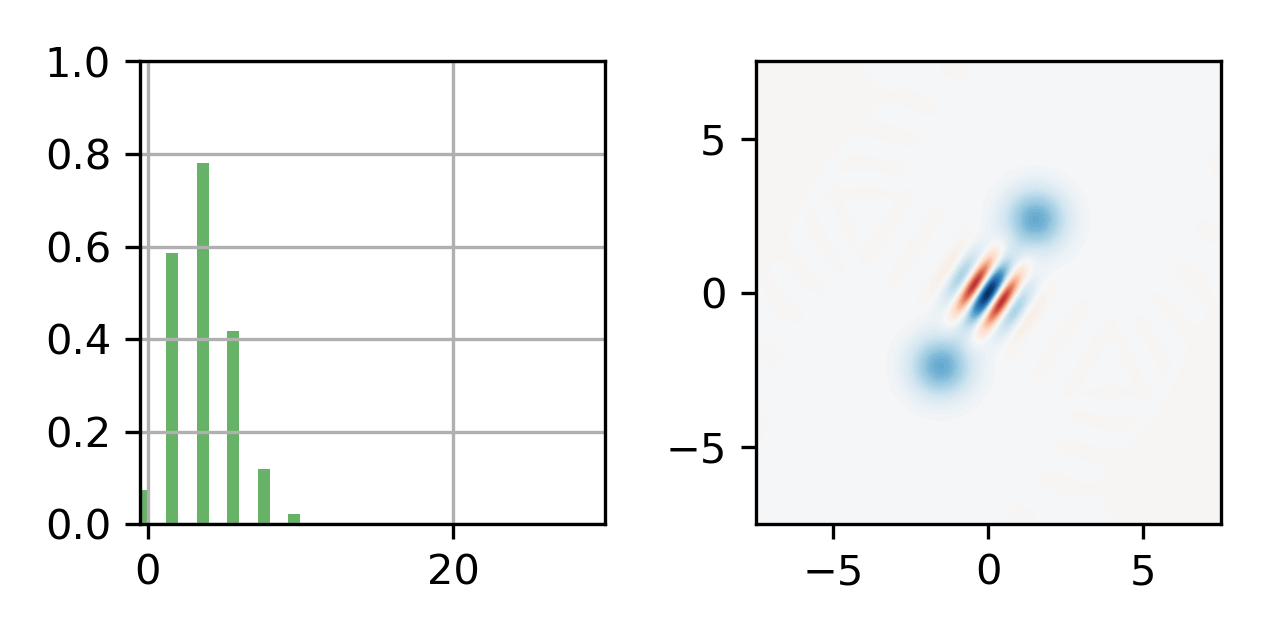
\includegraphics[width=0.7\linewidth]{pres_wigner_cat}
\caption{État de chat avec l'état cohérent précédent.}
\label{fig:preswignercat}
\end{figure}
\end{frame}

\section{Décohérence}

\begin{frame}{Décohérence d'un système quantique}
\framesubtitle{Apparition}
\begin{figure}
\centering
\begin{tikzpicture}[node distance = 4cm, auto]
    % Place nodes
    \node [rectangle, draw, fill=blue!20,text width=3 cm, text height =3cm,text centered, rounded corners] (env) {Environnement};
	\node [rectangle, draw, fill=red!20,text width=2 cm, text height =1cm,text centered, rounded corners,left of=env,node distance = 5 cm] (sys) {Système};
	\node [below of=sys,node distance=1.3cm,text width=2.5cm,text centered] (evol) {Évolution non unitaire};

	\path [draw,dashed] (env) -- node (coupl) {Couplage} (sys);
	\node [rectangle, draw, text width=8cm,text height = 4cm,  rounded corners, left of=env,node distance=2.25cm] (all) {};
	\node [below of=all,node distance=2.5cm] {Évolution unitaire};
\end{tikzpicture}
\end{figure}
Un état pur dont on prends la trace partielle devient un état mixte.
\end{frame}

\begin{frame}{Décohérence d'un système quantique}
\framesubtitle{Matrice de densité}
\begin{block}{Matrice de densité}
\[
\rho=\sum p_{\alpha} \ket{\psi_{\alpha}}\bra{\psi_{\alpha}}
\]
Représente un mélange statistique d'états purs.
\end{block}
Pas une superposition:
\begin{figure}
\centering
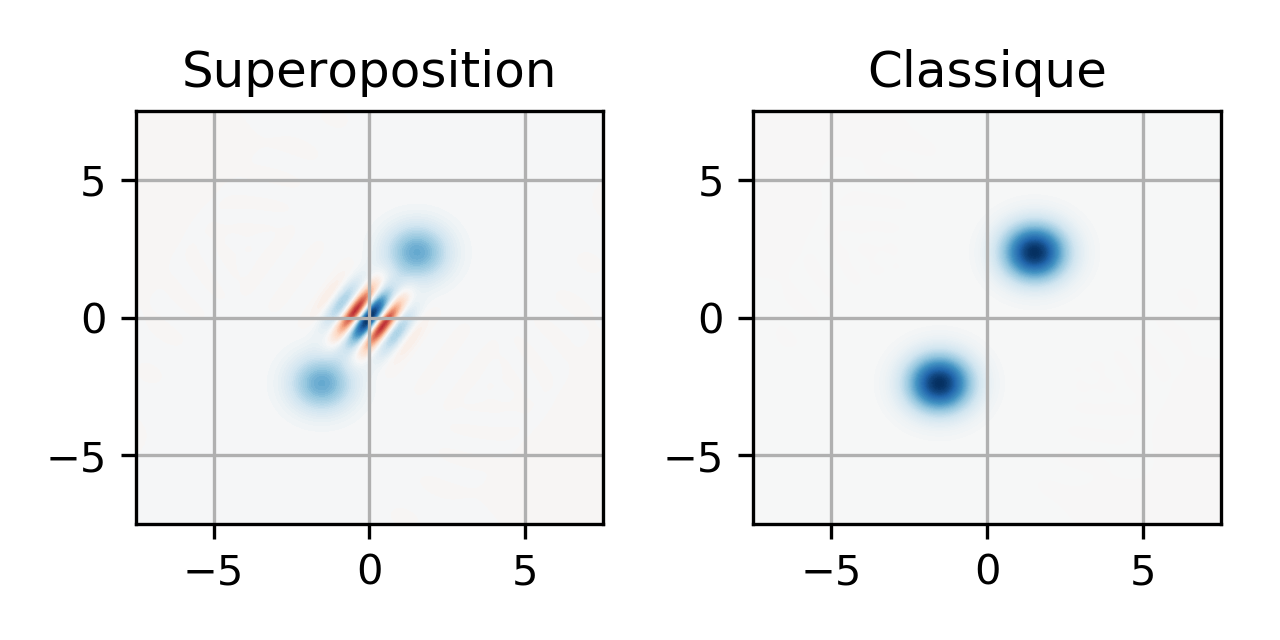
\includegraphics[width=0.6\linewidth]{pres_wigner_cat_dec}
\caption{A gauche un état de chat. A droite un mélange classique de deux états cohérents.}
\label{fig:preswignercatdec}
\end{figure}
\end{frame}

\begin{frame}{Équation de Lindblad}
\framesubtitle{Opérateurs de Kraus}

\end{frame}

\begin{frame}{Équation de Lindblad}
\framesubtitle{L'équation}
\begin{block}{Équation de Schrödinger}
\[
\frac{\textrm{d}\rho}{\textrm{dt}}=-\frac{i}{\hbar}\left[\mathcal{H},\rho\right]
\]
\end{block}
\begin{block}{Équation de Lindblad}
\[
\frac{\textrm{d}\rho}{\textrm{dt}}=-\frac{i}{\hbar}\left[\mathcal{H},\rho\right]+\sum_{\mu}\left(
	L_{\mu}\rho L_{\mu}^{\dag}-\frac 12 L_{\mu}^{\dag}L_{\mu}\rho -\frac 12 \rho L_{\mu}^{\dag}L_{\mu}
	\right)
\]
\end{block}
\end{frame}

\begin{frame}{Équation de Lindblad}
\framesubtitle{Signification physique}
Propriétés de l'équation:
\begin{enumerate}
\item Linéaire
\item Garde la trace de $\rho$ constante
\item Garde $\rho$ hermitienne

\end{enumerate}
\end{frame}

\begin{frame}{Équation de Lindblad}
\framesubtitle{Résolution avec QuTiP}
\end{frame}

\begin{frame}{Décohérence d'un qubit}
\framesubtitle{Canaux de décohérence}
\end{frame}

\begin{frame}{Décohérence d'un qubit}
\framesubtitle{Décohérence par perte d'énergie}
\end{frame}

\begin{frame}{Décohérence d'un qubit}
\framesubtitle{Décohérence par saut de phase}
\end{frame}


\begin{frame}{Décohérence d'un oscillateur}
\framesubtitle{Canal de décohérence}
\end{frame}

\begin{frame}{Décohérence d'un oscillateur}
\framesubtitle{État de Fock}
\end{frame}

\begin{frame}{Décohérence d'un oscillateur}
\framesubtitle{État cohérent}
\end{frame}

\begin{frame}{Décohérence d'un oscillateur}
\framesubtitle{État de chat}
\end{frame}

\begin{frame}{Entropie}
content...
\end{frame}

\section{Trajectoires quantiques et mesures}

\begin{frame}{Trajectoires quantiques et mesures}
\framesubtitle{Une autre approche a la décohérence}
\end{frame}

\begin{frame}{Trajectoire d'un qubit}
\framesubtitle{Perte d'énergie}
\end{frame}

\begin{frame}{Trajectoire d'un qubit}
\framesubtitle{Perte de phase}
\end{frame}

\begin{frame}{Trajectoire d'un oscillateur}
\framesubtitle{Décohérence d'un état de Fock}
\end{frame}

\begin{frame}{Trajectoire d'un oscillateur}
\framesubtitle{Décohérence d'un état cohérent}
\end{frame}


\begin{frame}{Trajectoire d'un qubit couplé a un oscillateur}
\framesubtitle{Décohérence d'un état de Fock}
\end{frame}

\begin{frame}{Conclusion}
content...
\end{frame}

\begin{frame}[plain]
\begin{beamercolorbox}[sep=8pt,center]{title}
\usebeamerfont{title}Remerciements%
\end{beamercolorbox}
\centering
Nous tenons à remercier Quentin Ficheux pour son aide précieuse et ses explications très claires. %\\\vspace{2cm}
%\[\star\hspace{1em}\star\hspace{1em}\star\]
%\pgfornament[width=3cm,color=green!20!black]{75}

\end{frame}

\appendix
\setbeamertemplate{footline}{}

\begin{frame}
\vfill
\begin{beamercolorbox}[sep=8pt,center]{title}
\usebeamerfont{title}Annexe
\end{beamercolorbox}
\vfill
\end{frame}

\begin{frame}{Résolution analytique}
\framesubtitle{Qubit (Annexe)}
L'hamiltonien doit être hermitien. On peut le décomposer donc sur la base des matrices de Pauli:\vspace{1em}
\begin{columns}
\column{0.25\textwidth}
\centering
id\\\vspace{1em}
$\begin{bmatrix}1&0\\0&1\end{bmatrix}$
\column{0.25\textwidth}
\centering
$\sigma_x$\\\vspace{1em}
$\begin{bmatrix}0&1\\1&0\end{bmatrix}$
\column{0.25\textwidth}
\centering
$\sigma_y$\\\vspace{1em}
$\begin{bmatrix}0&-i\\i&0\end{bmatrix}$
\column{0.25\textwidth}
\centering
$\sigma_z$\\\vspace{1em}
$\begin{bmatrix}1&0\\0&-1\end{bmatrix}$
\end{columns}\vspace{1em}
On a \[H=E_0\cdot id+\vec{r}\cdot\vec{\sigma}\]
\end{frame}

\end{document}
